\chapter{Design and characterization of basic RTL blocks}
\label{chapter:rtl}

\section{Scalar RTL blocks}

This work provides characterized RTL blocks for:

\begin{itemize}
    \item Arithmetic

    \begin{itemize}
        \item Adder
        \item Subtractor
        \item Multiplier
    \end{itemize}
    
    \item Comparison

    \begin{itemize}
        \item Equality comparator
    \end{itemize}
\end{itemize}

These straightforward circuits are useful as building blocks for other RTL designs, and the characterization metrics for these circuits are useful building-blocks for modeling.

These components are parameterized by operand bitwidth. All of these components are scalar, processing one set of operands per cycle and producing one output.

\section{Vectorized RTL blocks}

All ``vectorized' RTL blocks consume vector inputs and yield vector outputs. Depending on implementation, the degree of input and output vectorization may be determined by separate parameters (as is the case for the ``skip-ahead'' intersection unit) or by a single parameter (as is the case for the two-fingered merge-based intersection unit.)

Here, ``vectorization'' is used to mean that (1) the input and output data structures of the RTL block are vectors, and (2) the processing throughput is such that all vector operands are consumed within a cycle, and each vector output is produced in its entirety within a cycle.

Notably, an RTL block being ``vectorized'' is decoupled from the degree of parallelism of the underlying combinational logic. The vectorized ripple prefix-sum, for example, uses a linear-depth design based on chained adders in order to process a vector of inputs within a cycle (provided that the critical path latency complies with the clock latency), while the vectorized parallel Kogge-Stone\cite{koggestone} prefix-sum uses a log-depth tree design that trades off higher area for sub-linear critical path length scaling.

\subsection{Prefix-sum units}

\textbf{Vectorized prefix sum parameters:}

\begin{itemize}
    \item Input vector length
    \item Word bits
\end{itemize}

\textbf{RTL implementations for the following prefix sum designs (all sharing the above parameter list) are provided:}

\begin{itemize}
    \item \textbf{Ripple prefix-sum:} linear-depth prefix-sum implementation based on chained adders.
    \item \textbf{Parallel Kogge-Stone\cite{koggestone} prefix-sum:} log-depth prefix-sum implementation based on adder trees.
\end{itemize}

\subsubsection{Kogge-Stone prefix-sum}

\begin{figure}[H]
    \centering
    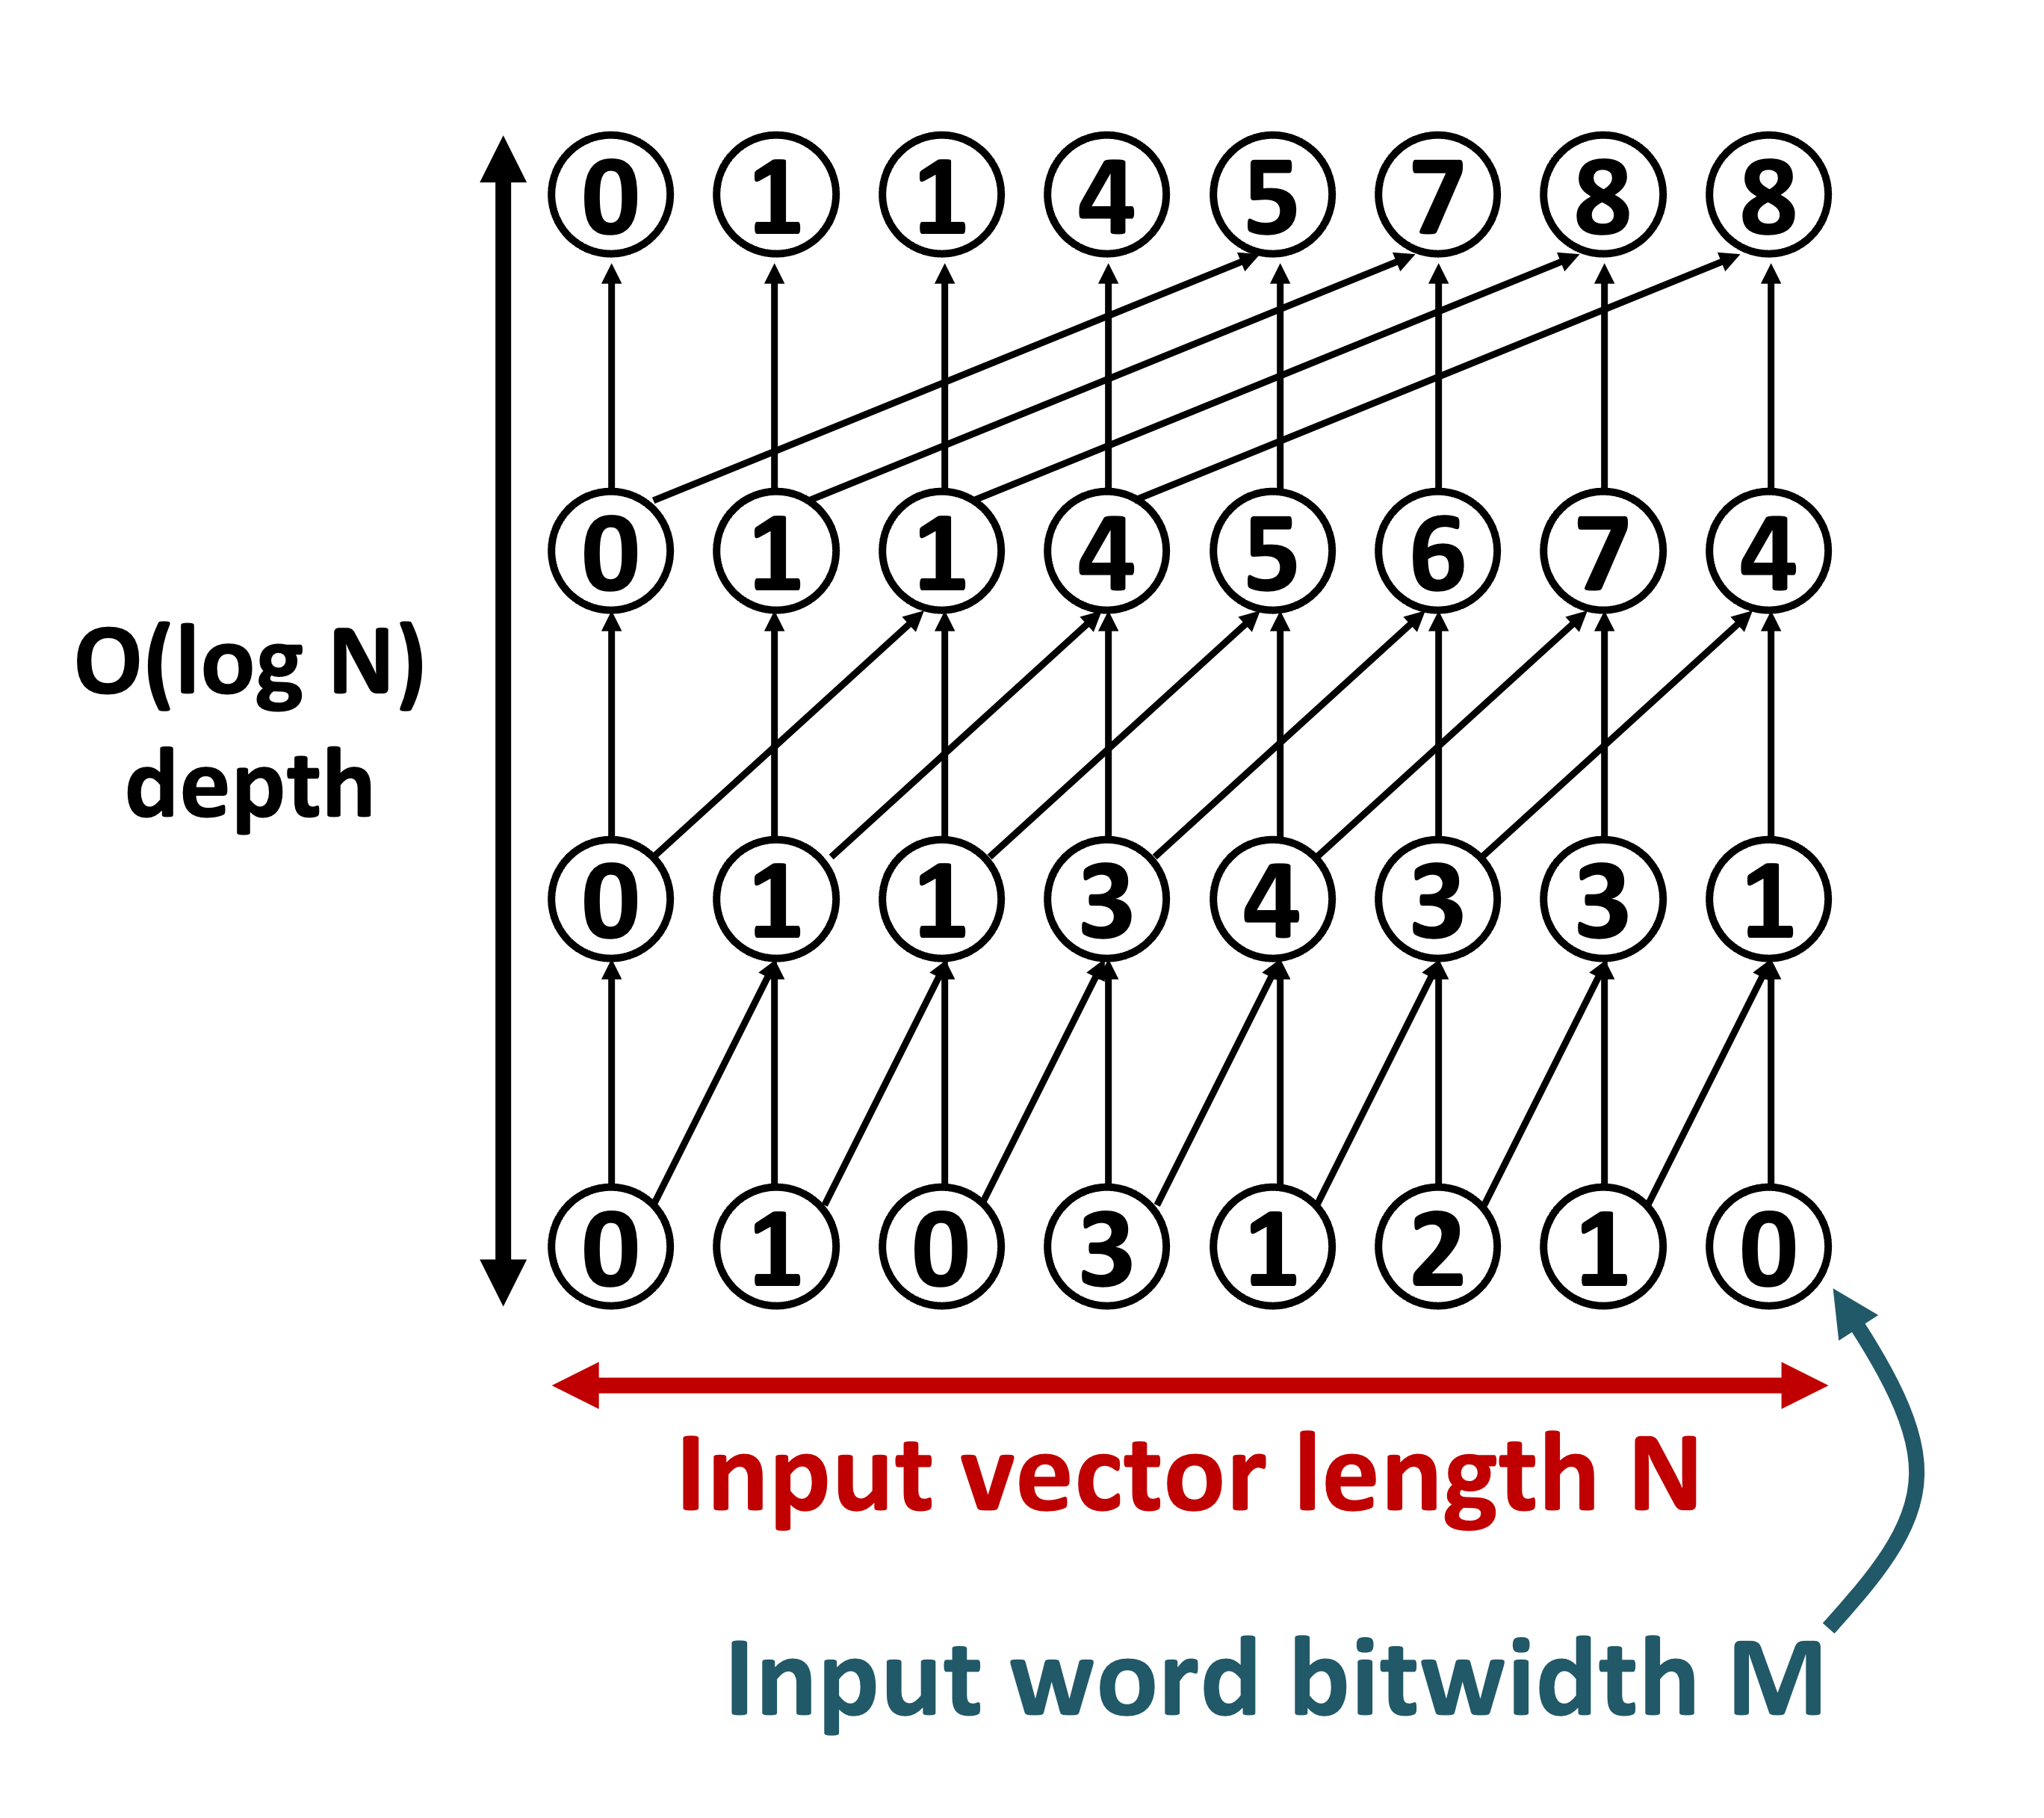
\includegraphics[width=0.95\textwidth]{figures/kogge_stone_prefix_sum.png}
    \caption{The Kogge-Stone\cite{koggestone} prefix-sum RTL block implements a log-depth vectorized prefix-sum with a 1-stage vector pipeline (registered I/O.) It is parameterized by \textbf{input word bitwidth} and \textbf{degree of vectorization.}}
    \label{fig:kogge_stone_prefix_sum}
\end{figure}

\subsubsection{Ripple prefix-sum}


\begin{figure}[H]
    \centering
    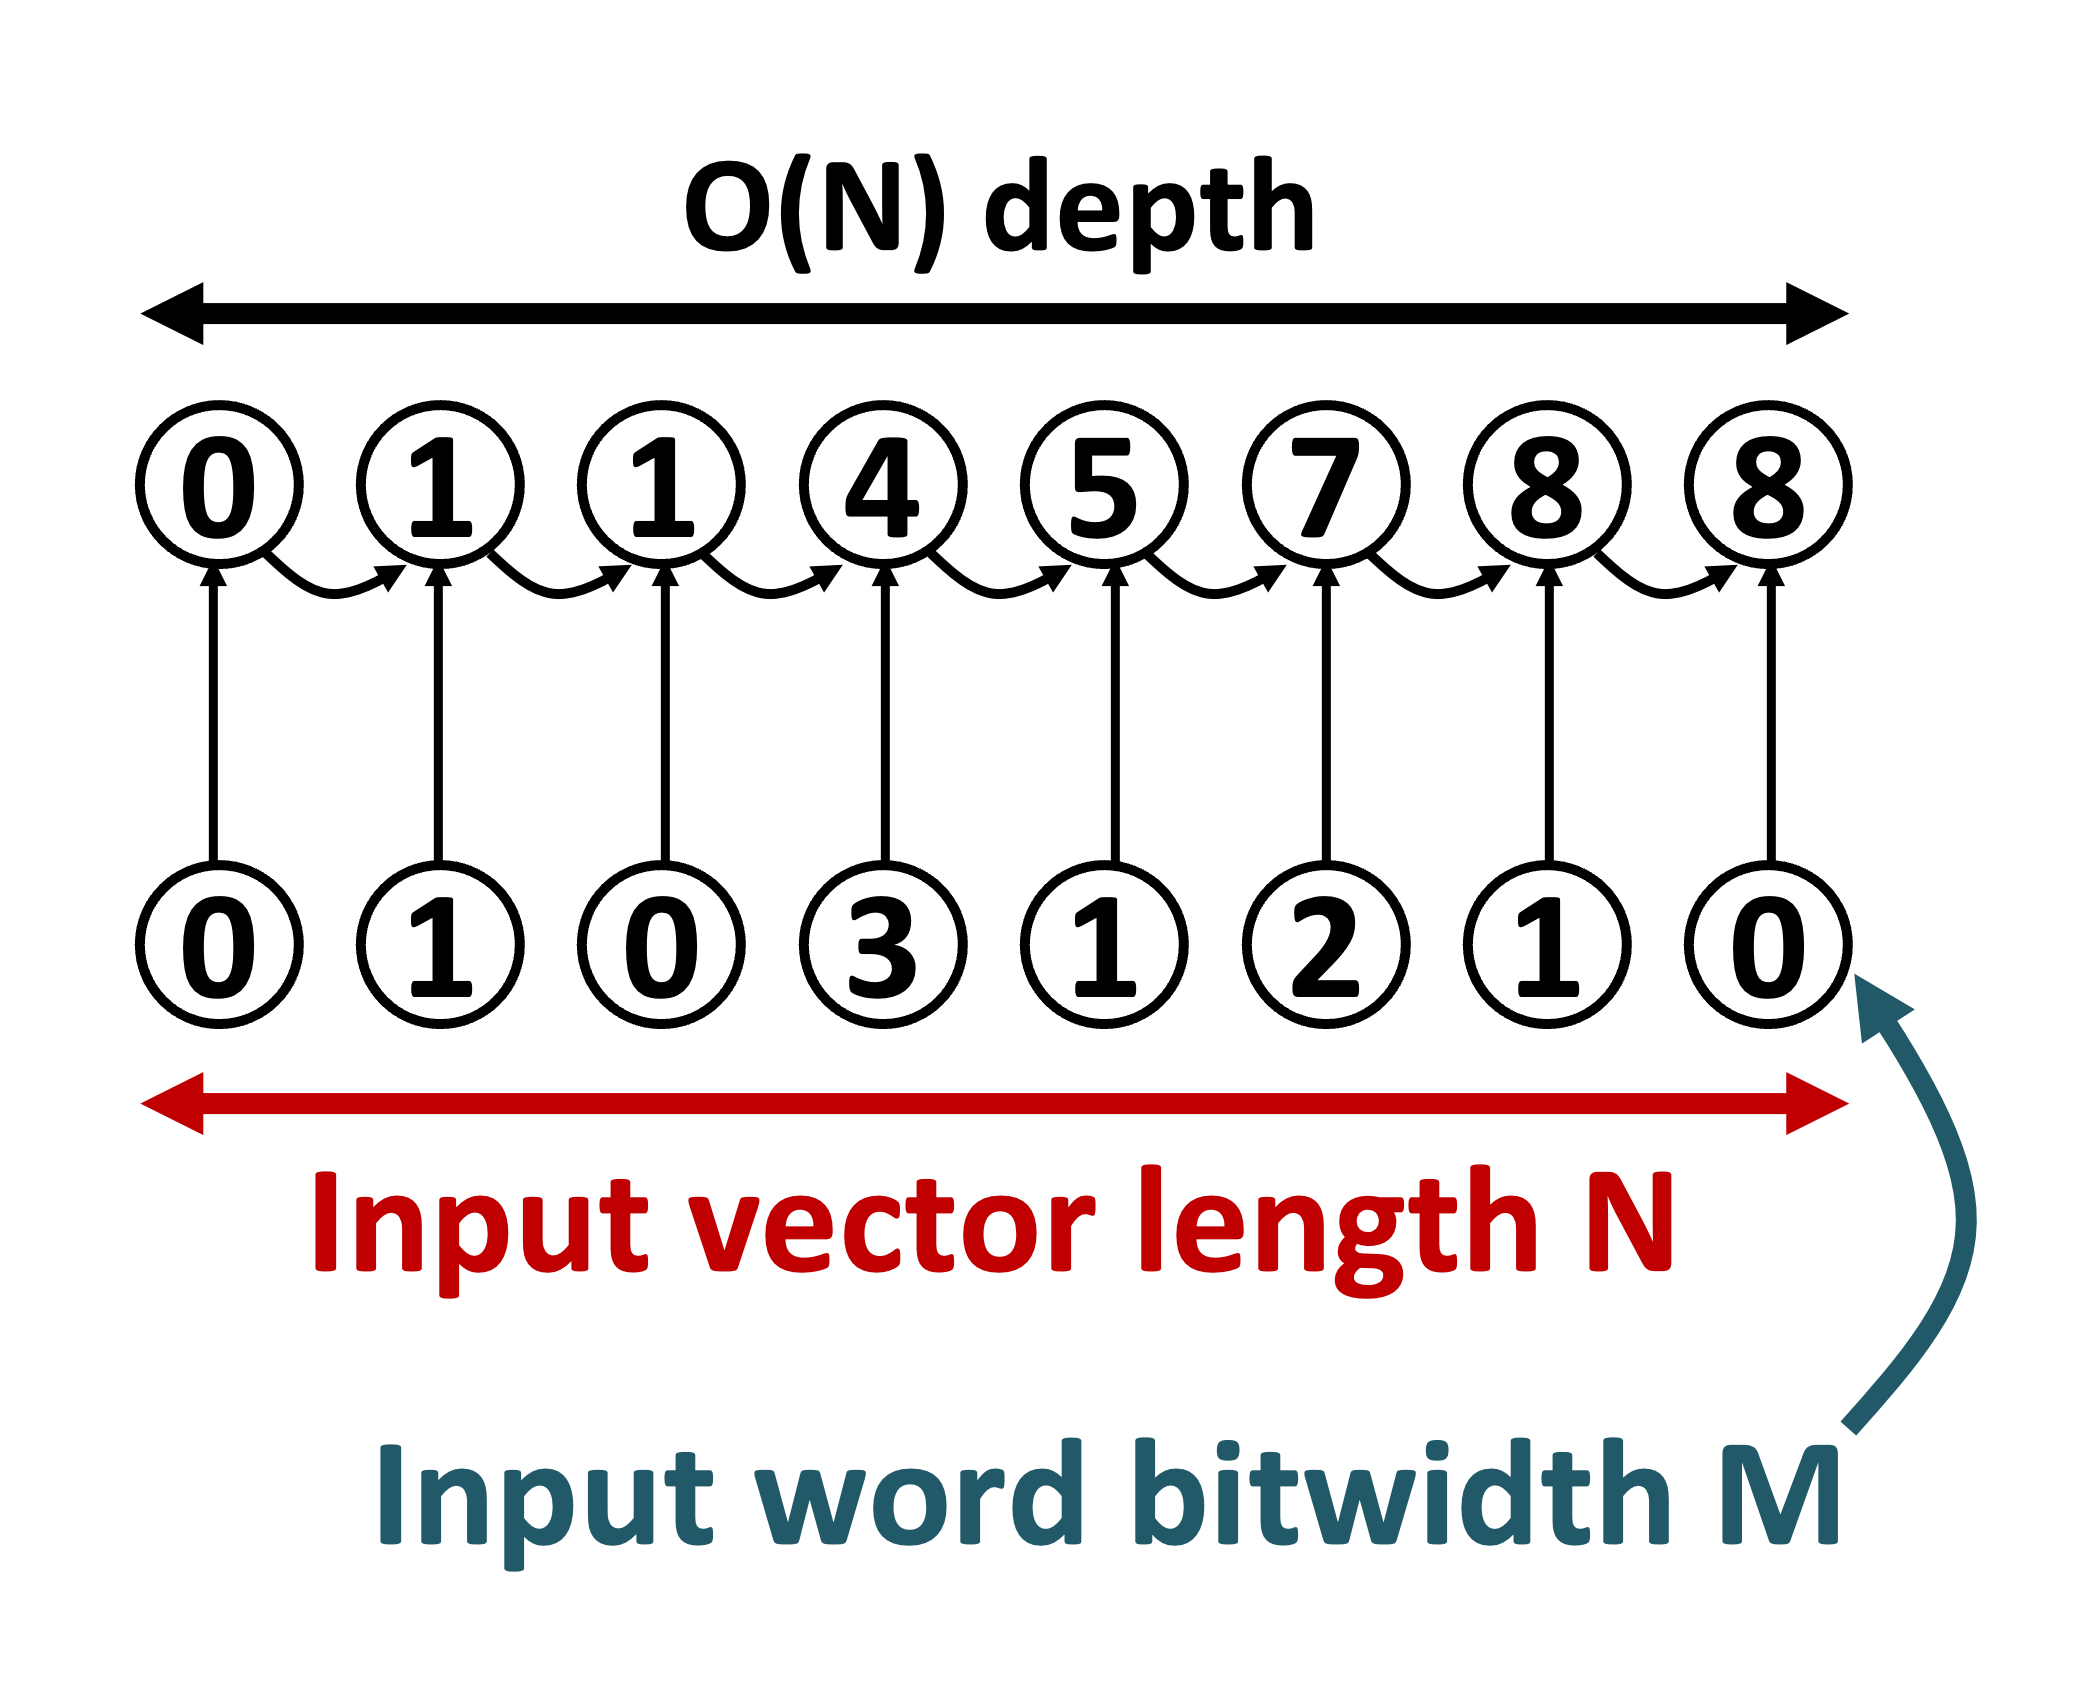
\includegraphics[width=0.95\textwidth]{figures/ripple_prefix_sum.png}
    \caption{The ripple prefix-sum RTL block implements a linear-depth vectorized prefix-sum. It is parameterized by \textbf{input word bitwidth} and \textbf{degree of vectorization.} This RTL block is implemented as a 1-stage vector pipeline (registered I/O) however the combinational design is not ``parallel'' and propagation delay is linear in the degree of vectorization.}
    \label{fig:ripple_prefix_sum}
\end{figure}
\subsection{Priority encoder units}

\textbf{Vector priority encoder parameters:}

\begin{itemize}
    \item Number of input bits
    \item Output vector size
    
    \begin{itemize}
        \item Meaning: if the output vector size is $k$, a vectorized priority encoder returns a vector of indices for the top-$k$ priority hot bits in the input vector. 
        \item If the input bitmask contains $n < k$ hot bits, the priority encoder returns a length-$k$ vector with the $n$ hot-bit indices compacted into the first $n$ vector elements; vector elements a offsets $>n-1$ are undefined.
    \end{itemize}

\end{itemize}

\textbf{RTL implementations for the following priority encoder designs (all sharing the above parameter list) are provided:}

\begin{itemize}
    \item \textbf{Parallel decimation-by-2 priority encoder\cite{recursive_priority_encoder}:} log-depth, decimation-by-2 parallel priority encoder design.
\end{itemize}

\subsection{Intersection units}

\subsubsection{Radix-2 merge-based intersection unit (``ExTensor-naive-like'')}

% Radix-2 intersection overview figure
\begin{figure}[H]
    \centering
    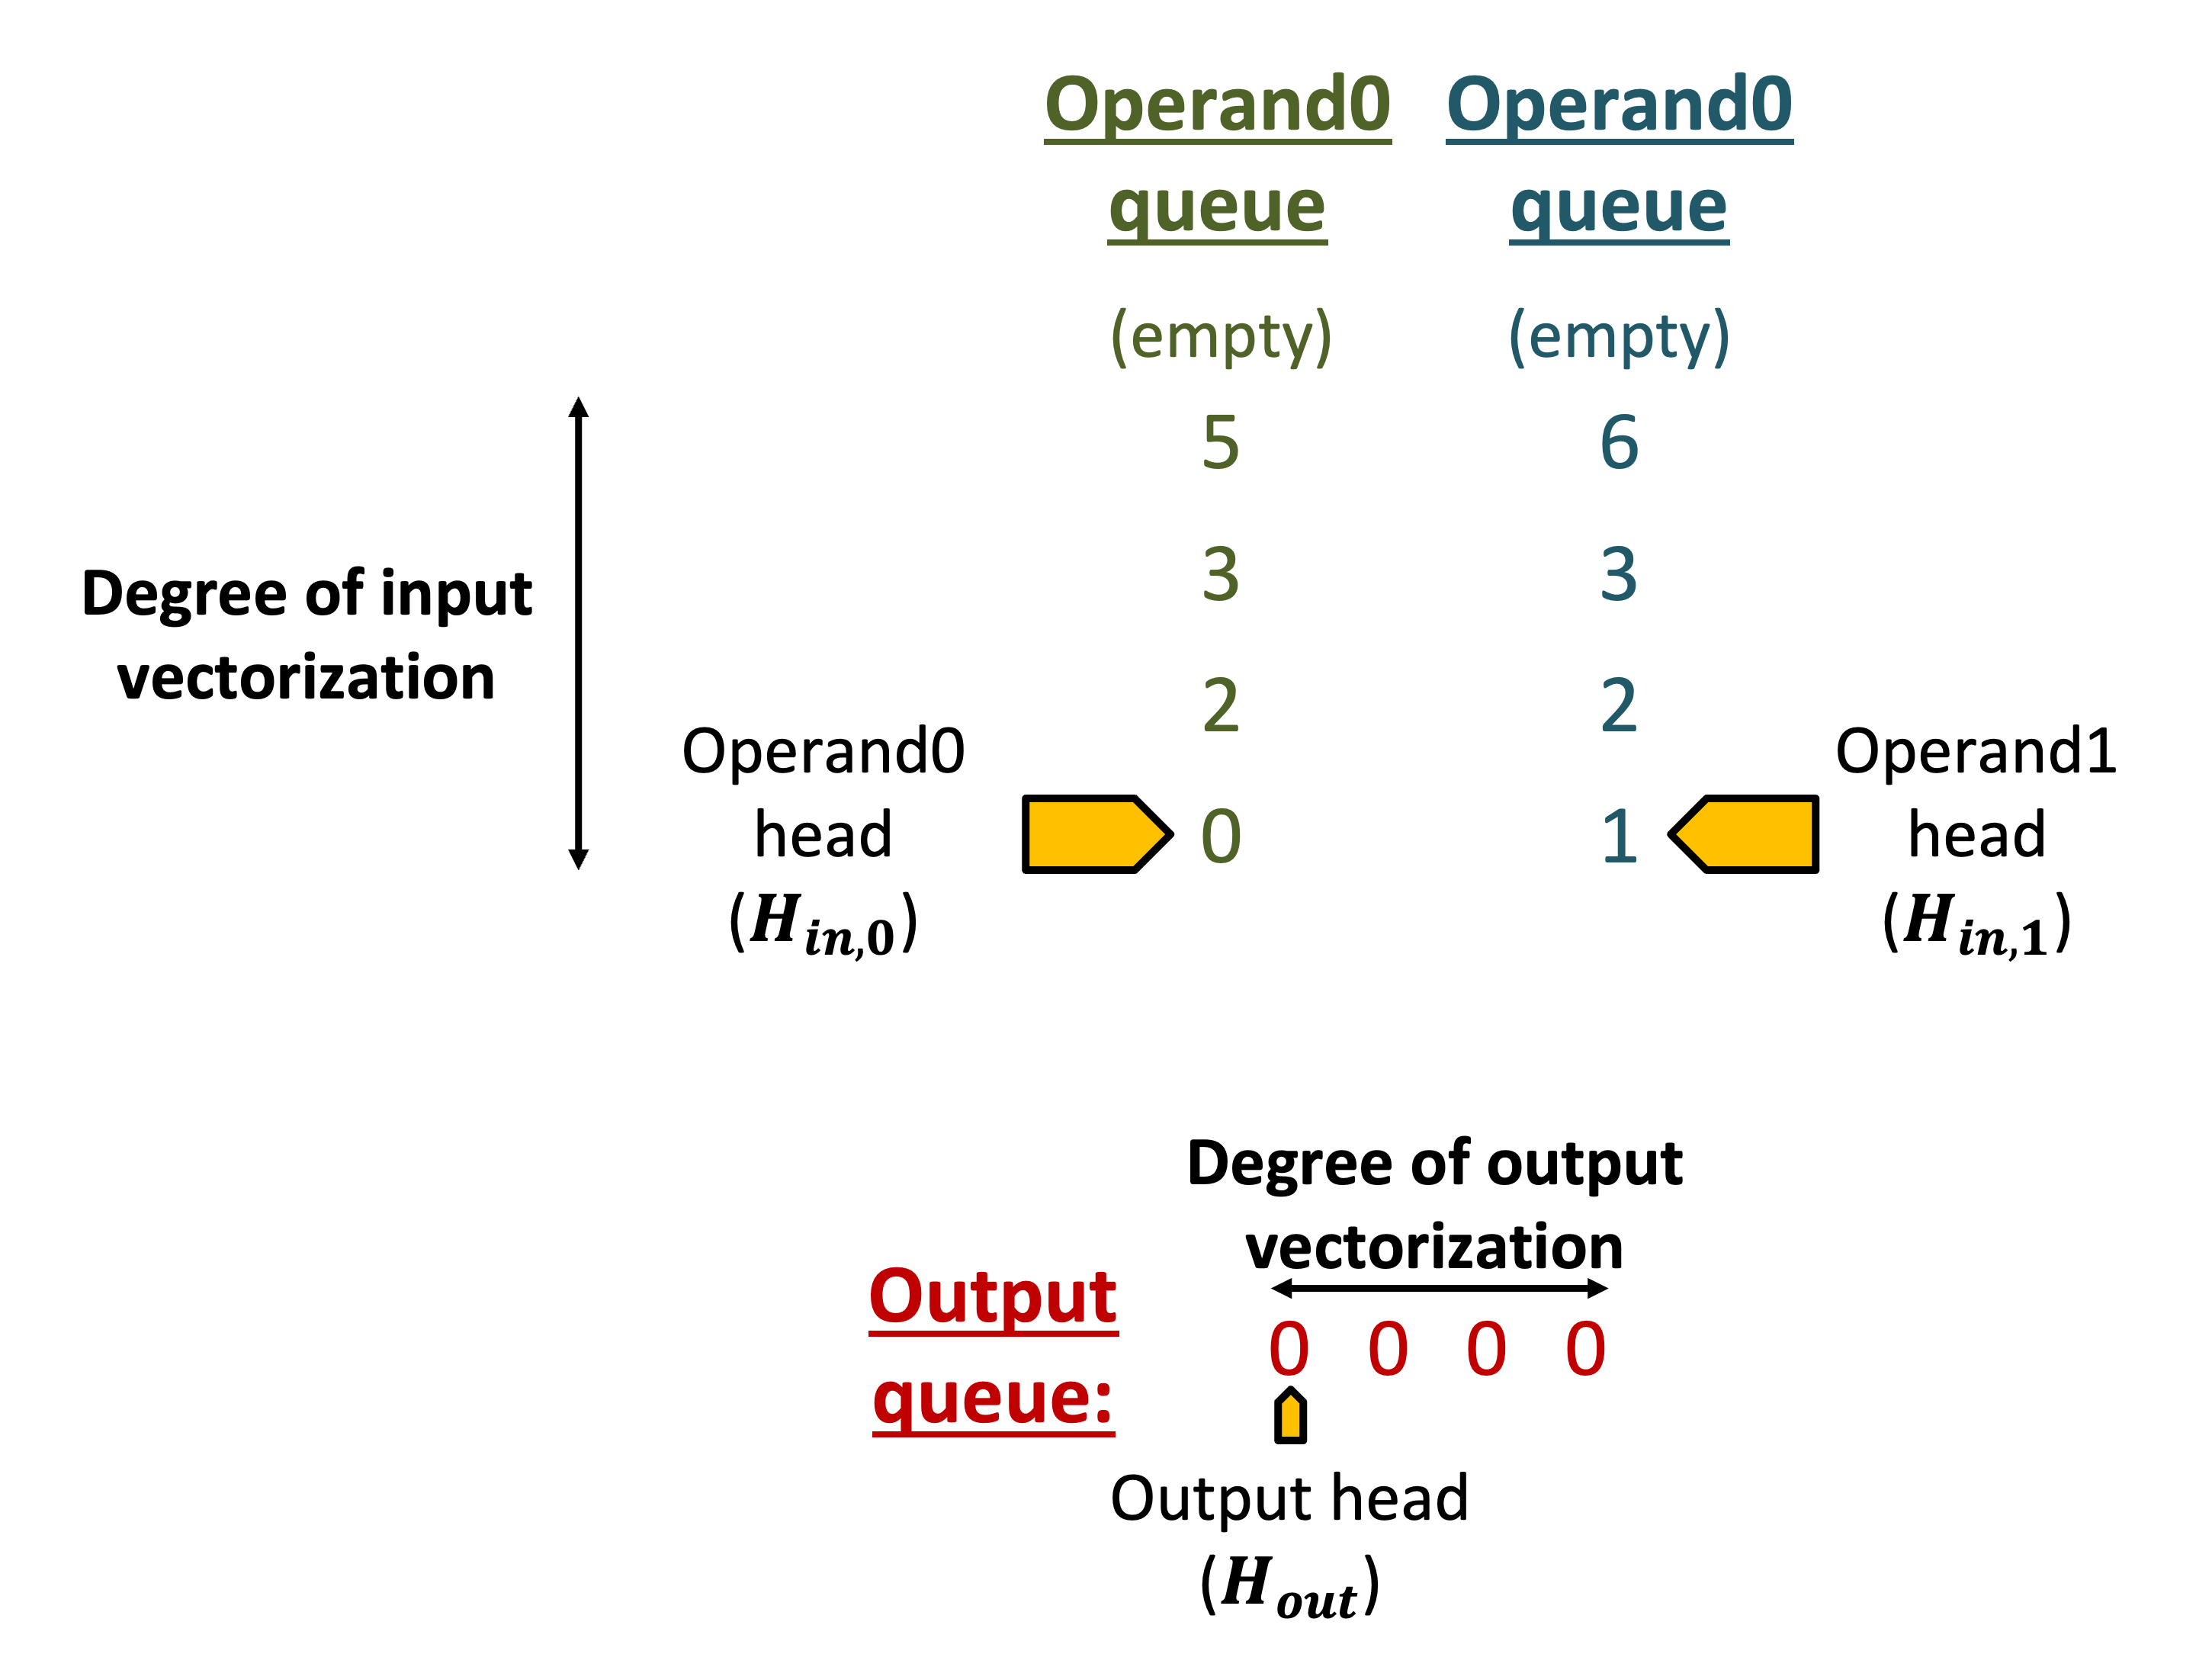
\includegraphics[width=\linewidth]{figures/radix2_intersect_overview.png}
    \caption{Overview of Radix2 Intersection}
    \label{fig:radix2-overview}
\end{figure}

% Radix-2 intersection example figure
\begin{figure}[H]
    \centering
    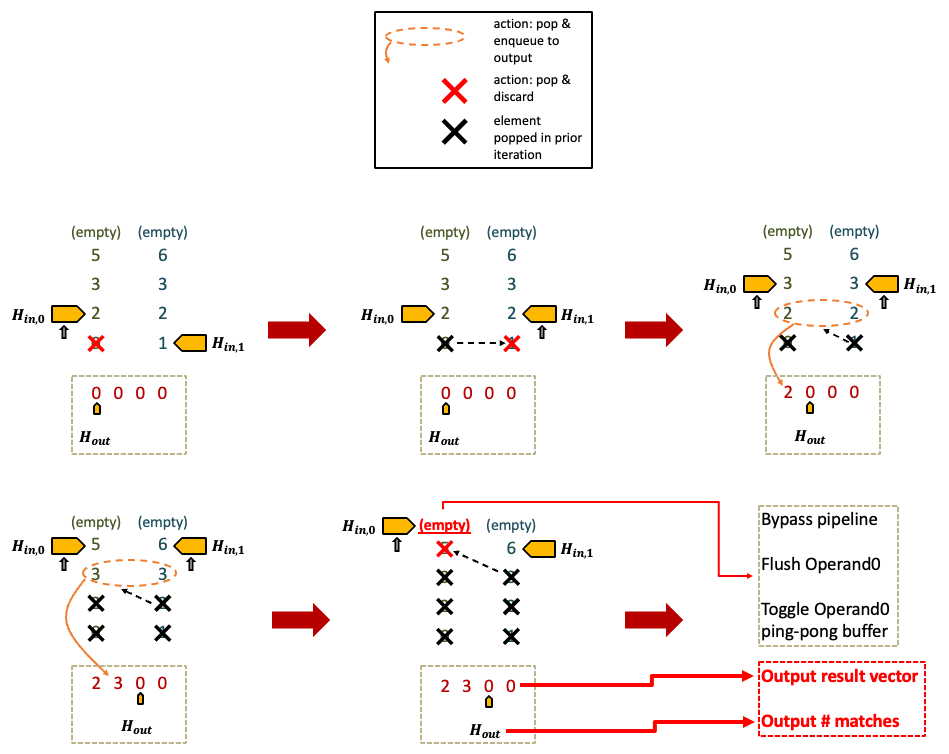
\includegraphics[width=\linewidth]{figures/radix2_intersect_example.png}
    \caption{Example of Radix2 Intersection}
    \label{fig:radix2-example}
\end{figure}

% Radix-2 intersection overview figure
\begin{figure}[H]
    \centering
    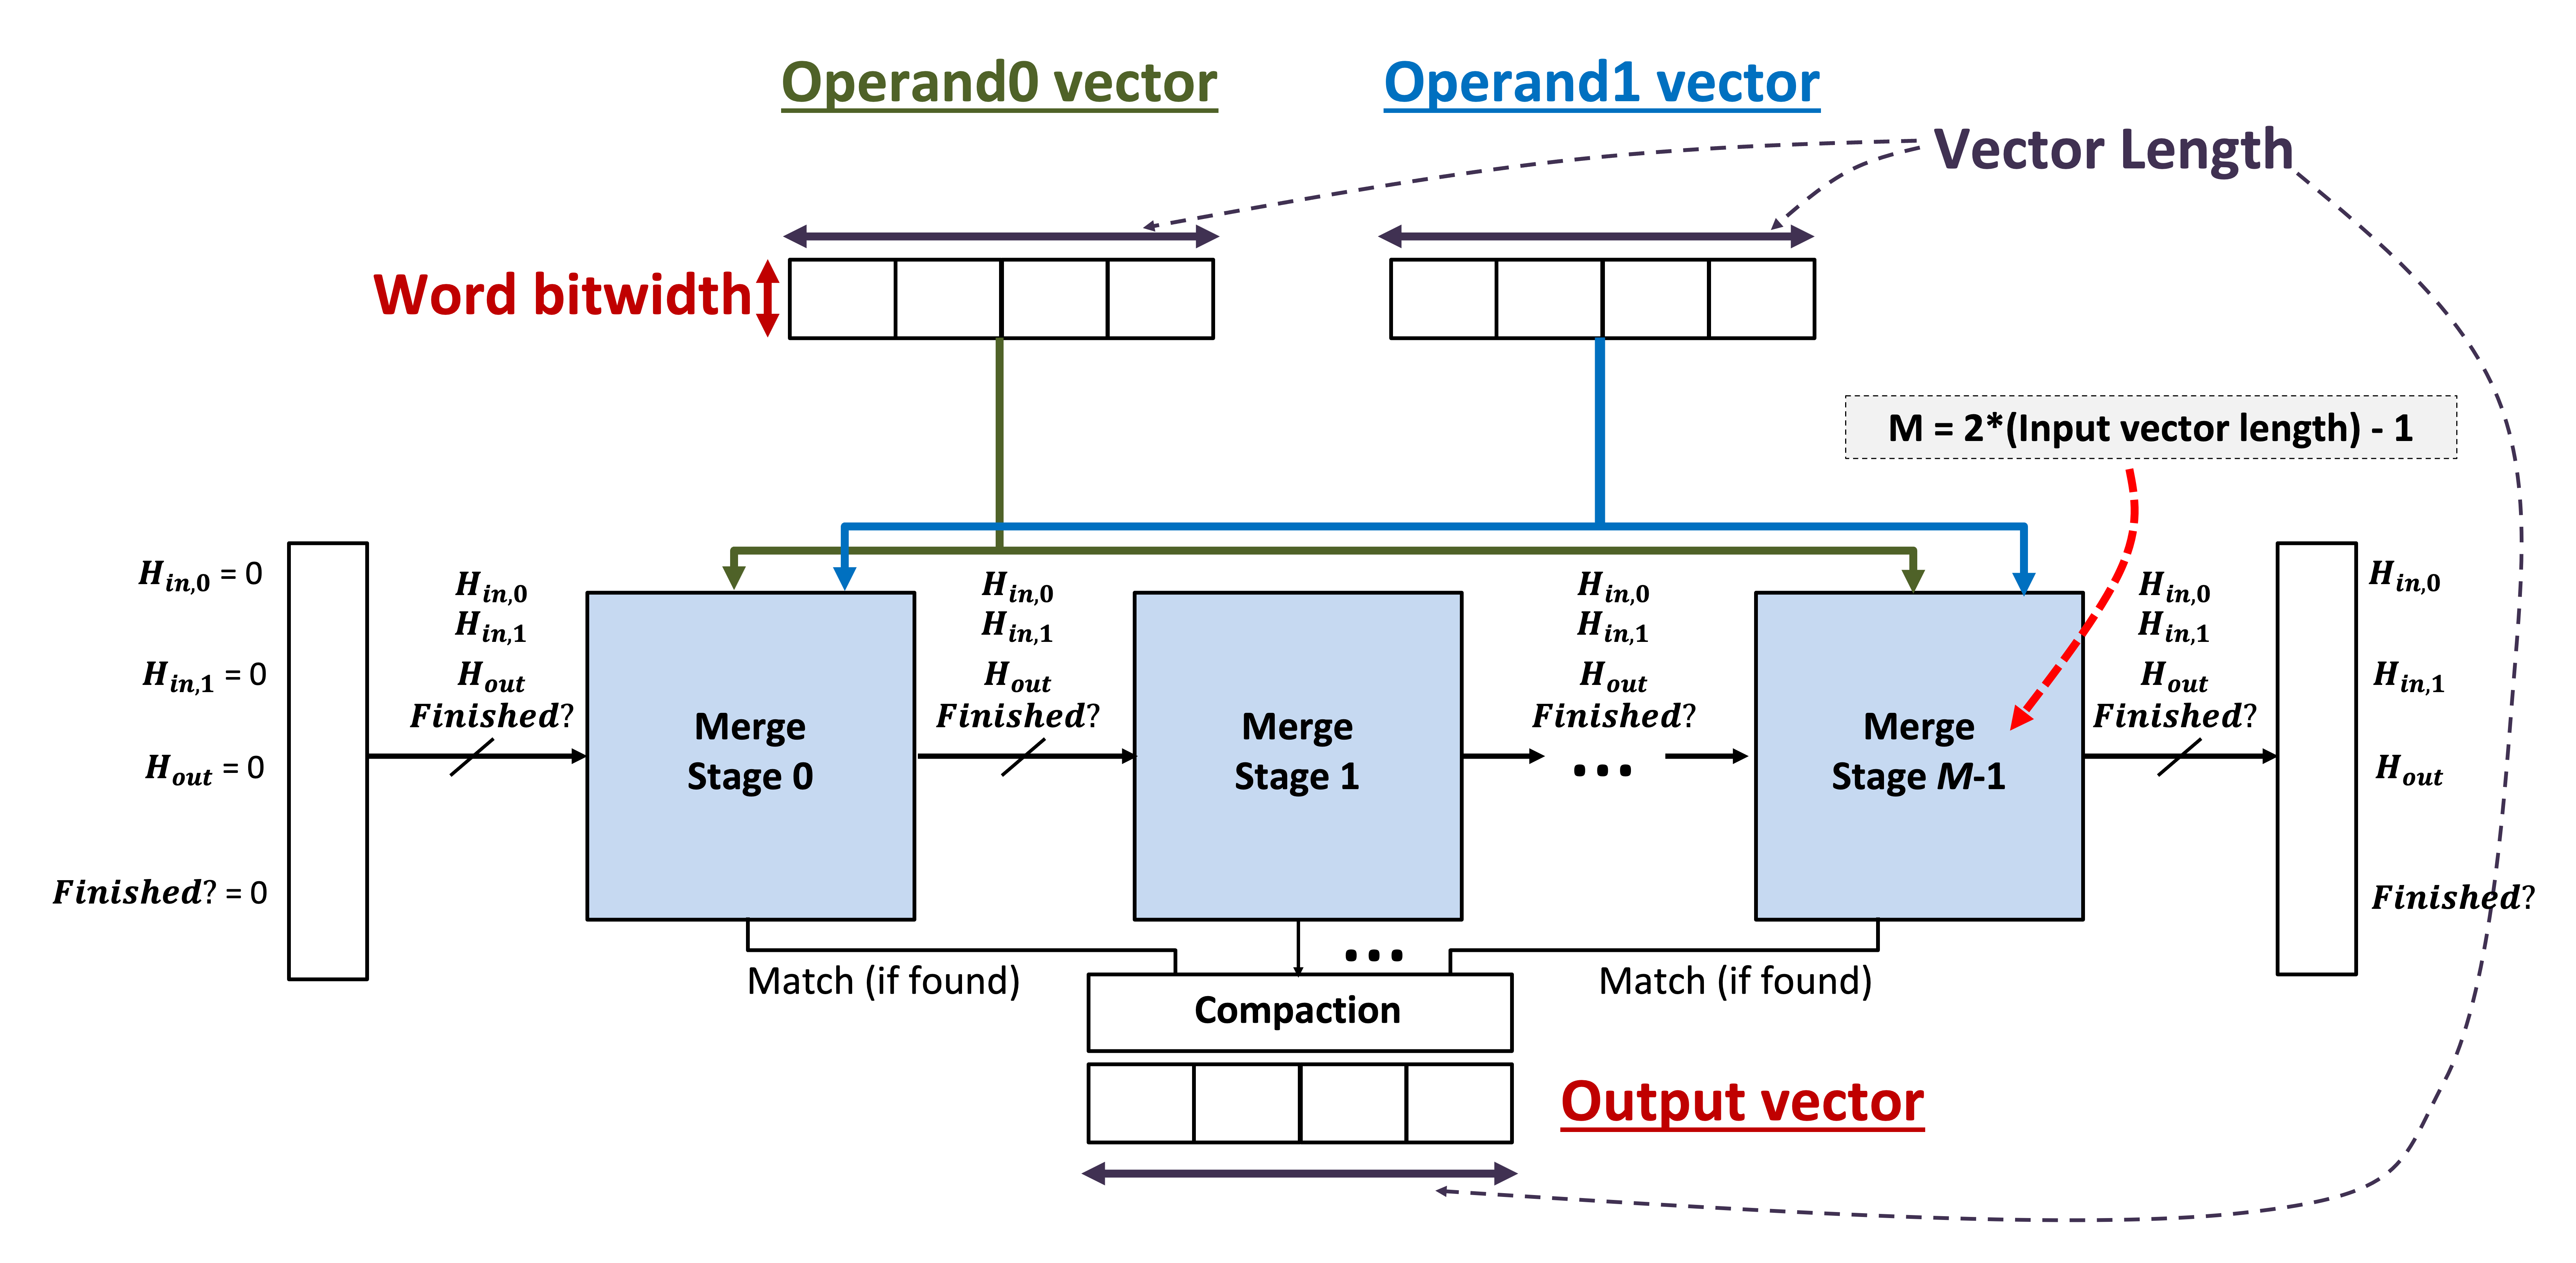
\includegraphics[width=\linewidth]{figures/two_finger_merge_pipeline.png}
    \caption{Radix-2 intersection vector pipeline}
    \label{fig:radix_2_vector pipeline}
\end{figure}

\subsubsection{``Skip-ahead'' intersection unit (``ExTensor-optimized-like'')}

\subsubsection{Parallel direct-mapped intersection unit}

This design intersects two vectors of sorted coordinate metadata, and outputs a third sorted vector of common metadata values between the two input vectors. See Figure~\ref{fig:direct_mapped_isect}.

The implementation is based on a ``direct-mapped approach'', analogous to direct-mapped cache. An array of decoders maps the input vector operands from position-space into coordinate-space; this mapping is performed in parallel. This yields two bitmasks (one per operand); in a given operand's bitmask, the index of each hot bit corresponds to an explicit coordinate value in the corresponding input vector. A bitmask intersection is then performed, yielding a new bit-vector in which each hot bit corresponds to a \textit{common} explicit coordinate value between the two vectors. Compaction logic maps these common coordinates back into position-space, yielding a sorted vector of explicit coordinate values which are common to both input vectors.

\textbf{Vectorized parallel direct-mapped intersection unit parameters:}

\begin{itemize}
    \item Vector size (applies to input and output.)
    \item Fiber size (the coordinate-space length of the two sparse fibers being intersected.)
    \item Coordinate metadata bitwidth.
\end{itemize}

For example, a fiber spanning the range of coordinate values $[0,L-1]$ would require the fiber size parameter to be set to L, regardless of the number of non-zero values in the fiber.

\begin{figure}[ht]
    \centering
    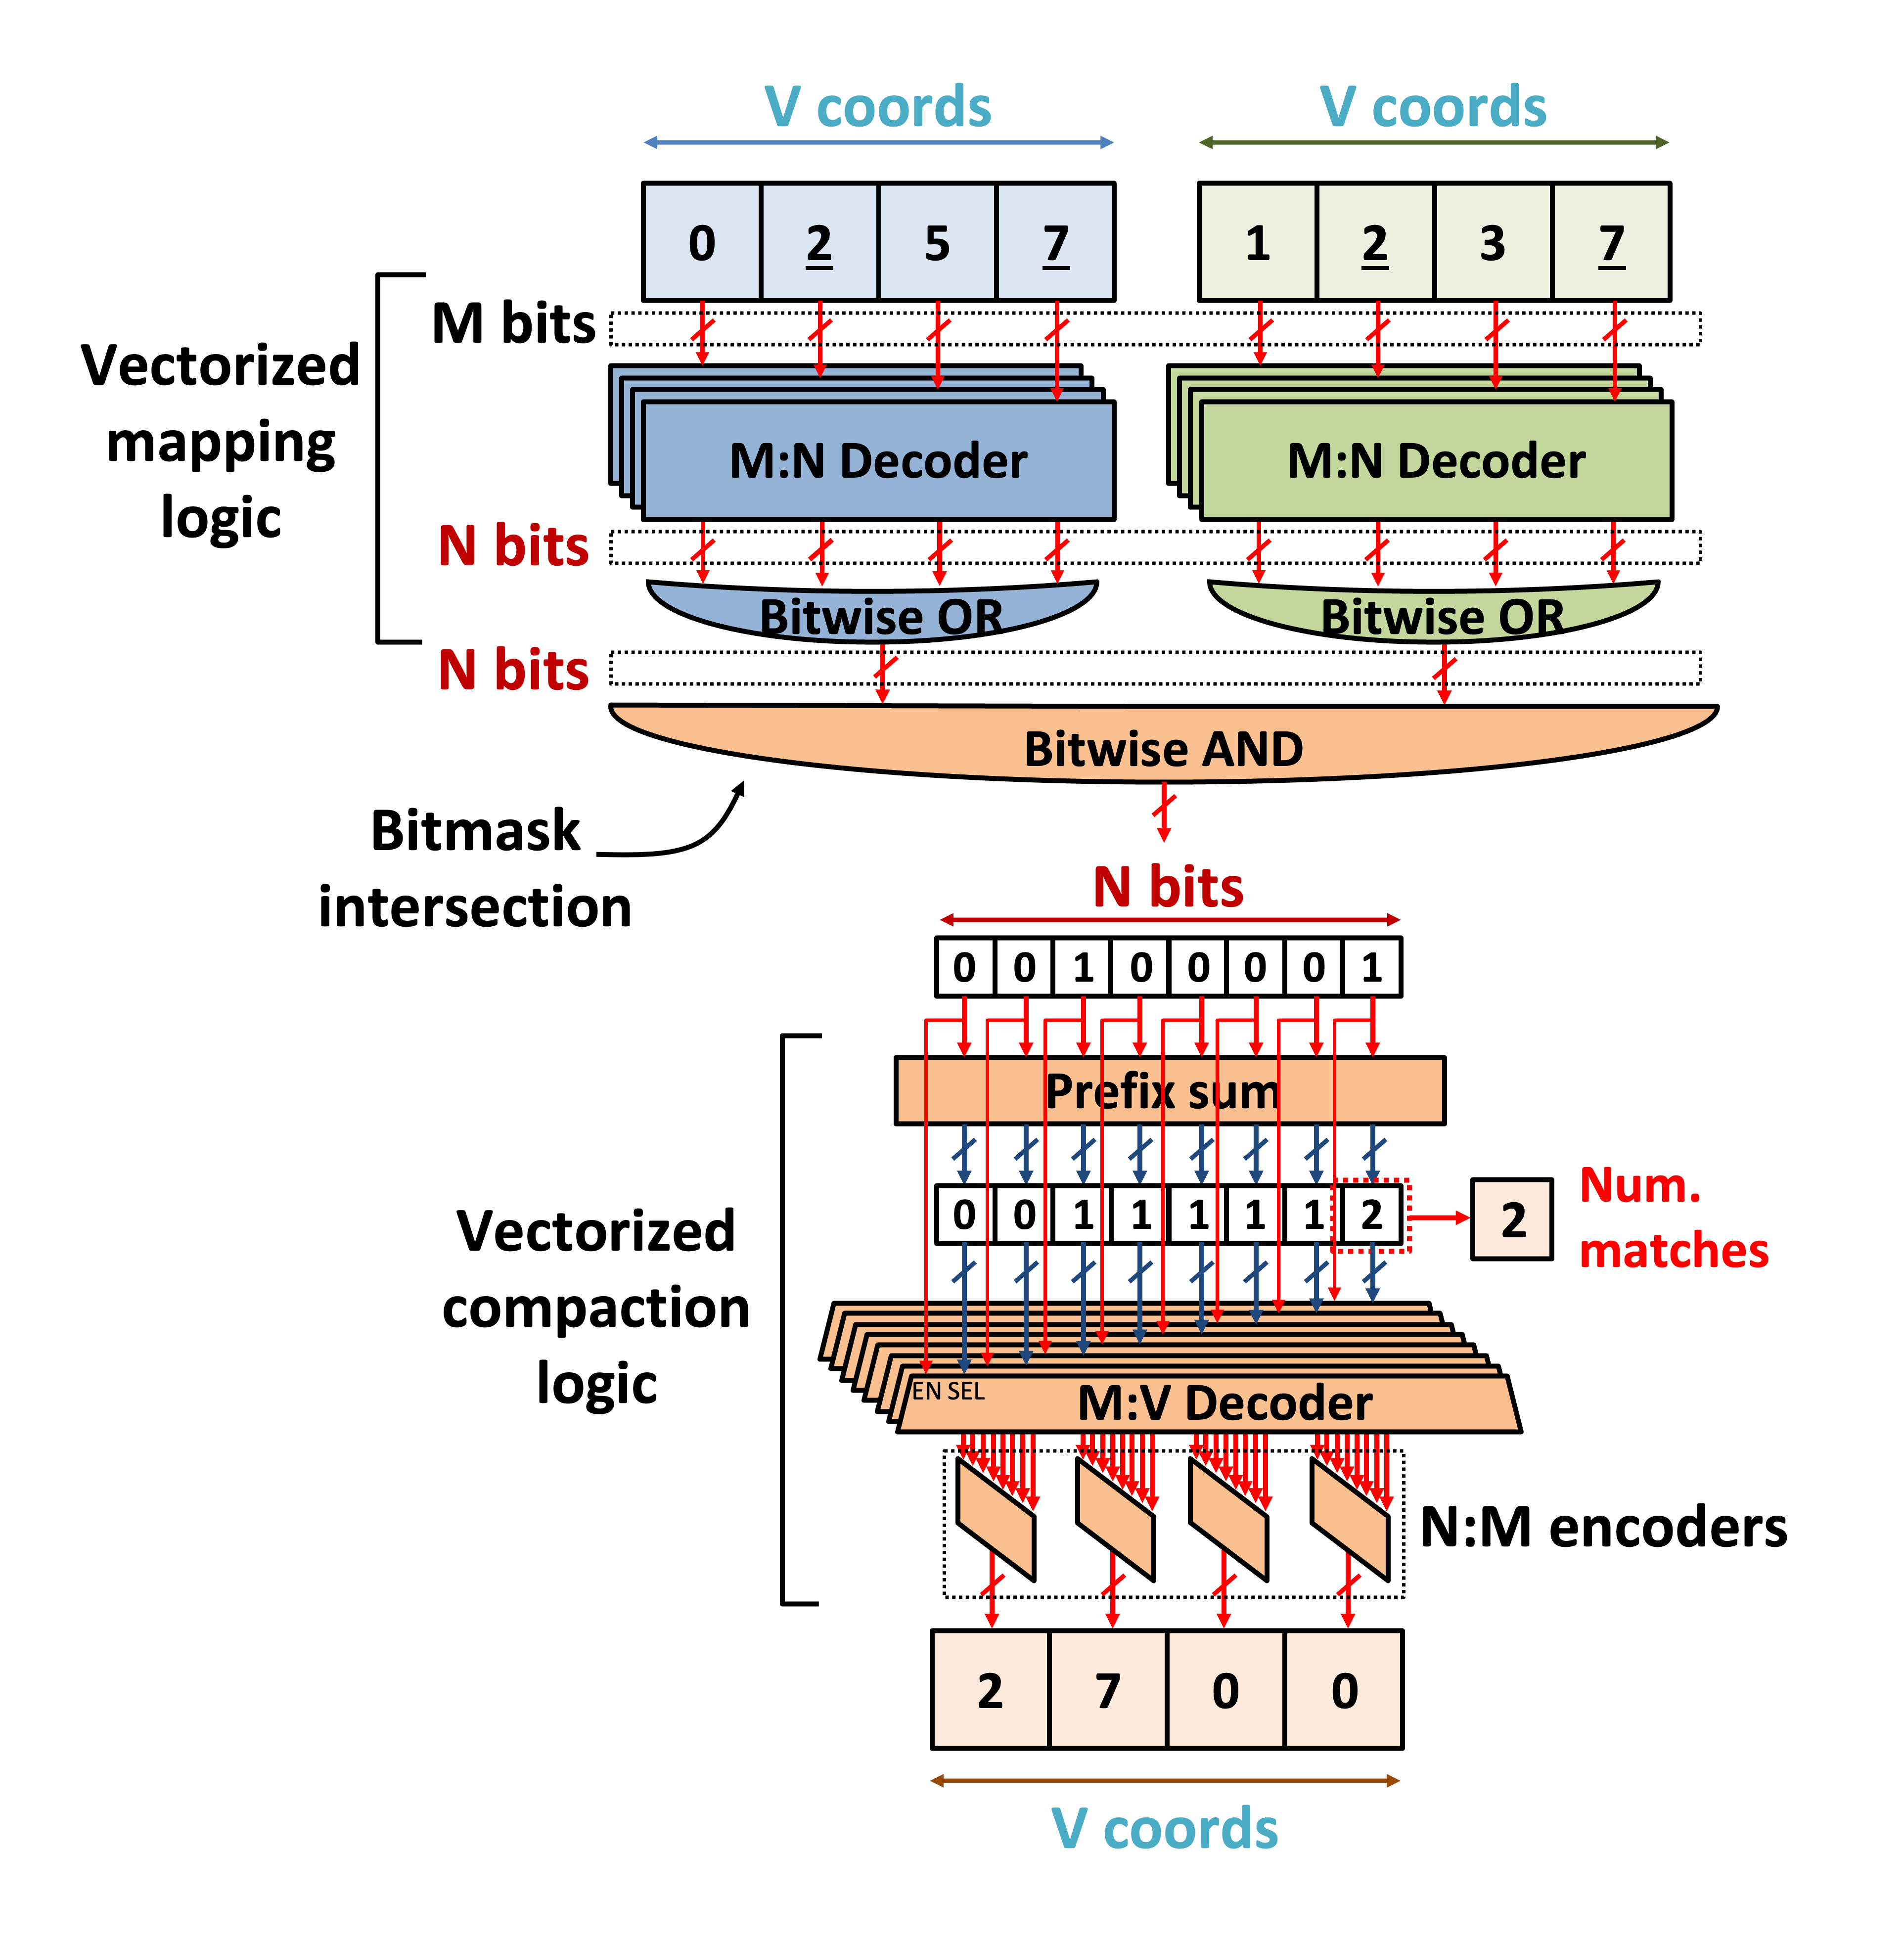
\includegraphics[width=0.95\textwidth]{figures/direct_mapped_isect.png}
    \caption{Vectorized direct-mapped intersection unit. Consumes two coordinate metadata vectors, and outputs a compacted and sorted vector of common elements, along with a count of common elements ($num\_matches$.) Output vector indices greater than $num\_matches - 1$ have undefined values.}
    \label{fig:direct_mapped_isect}
\end{figure}

\subsubsection{Parallel bitmask intersection unit}

\textbf{Vectorized parallel bitmask intersection unit parameters:}

\begin{itemize}
    \item Number of input bits
\end{itemize}

The parallel bitmask intersection unit applies a straightforward bitwise-AND operation and outputs the result.

% Bitmask intersection
\begin{figure}[H]
    \centering
    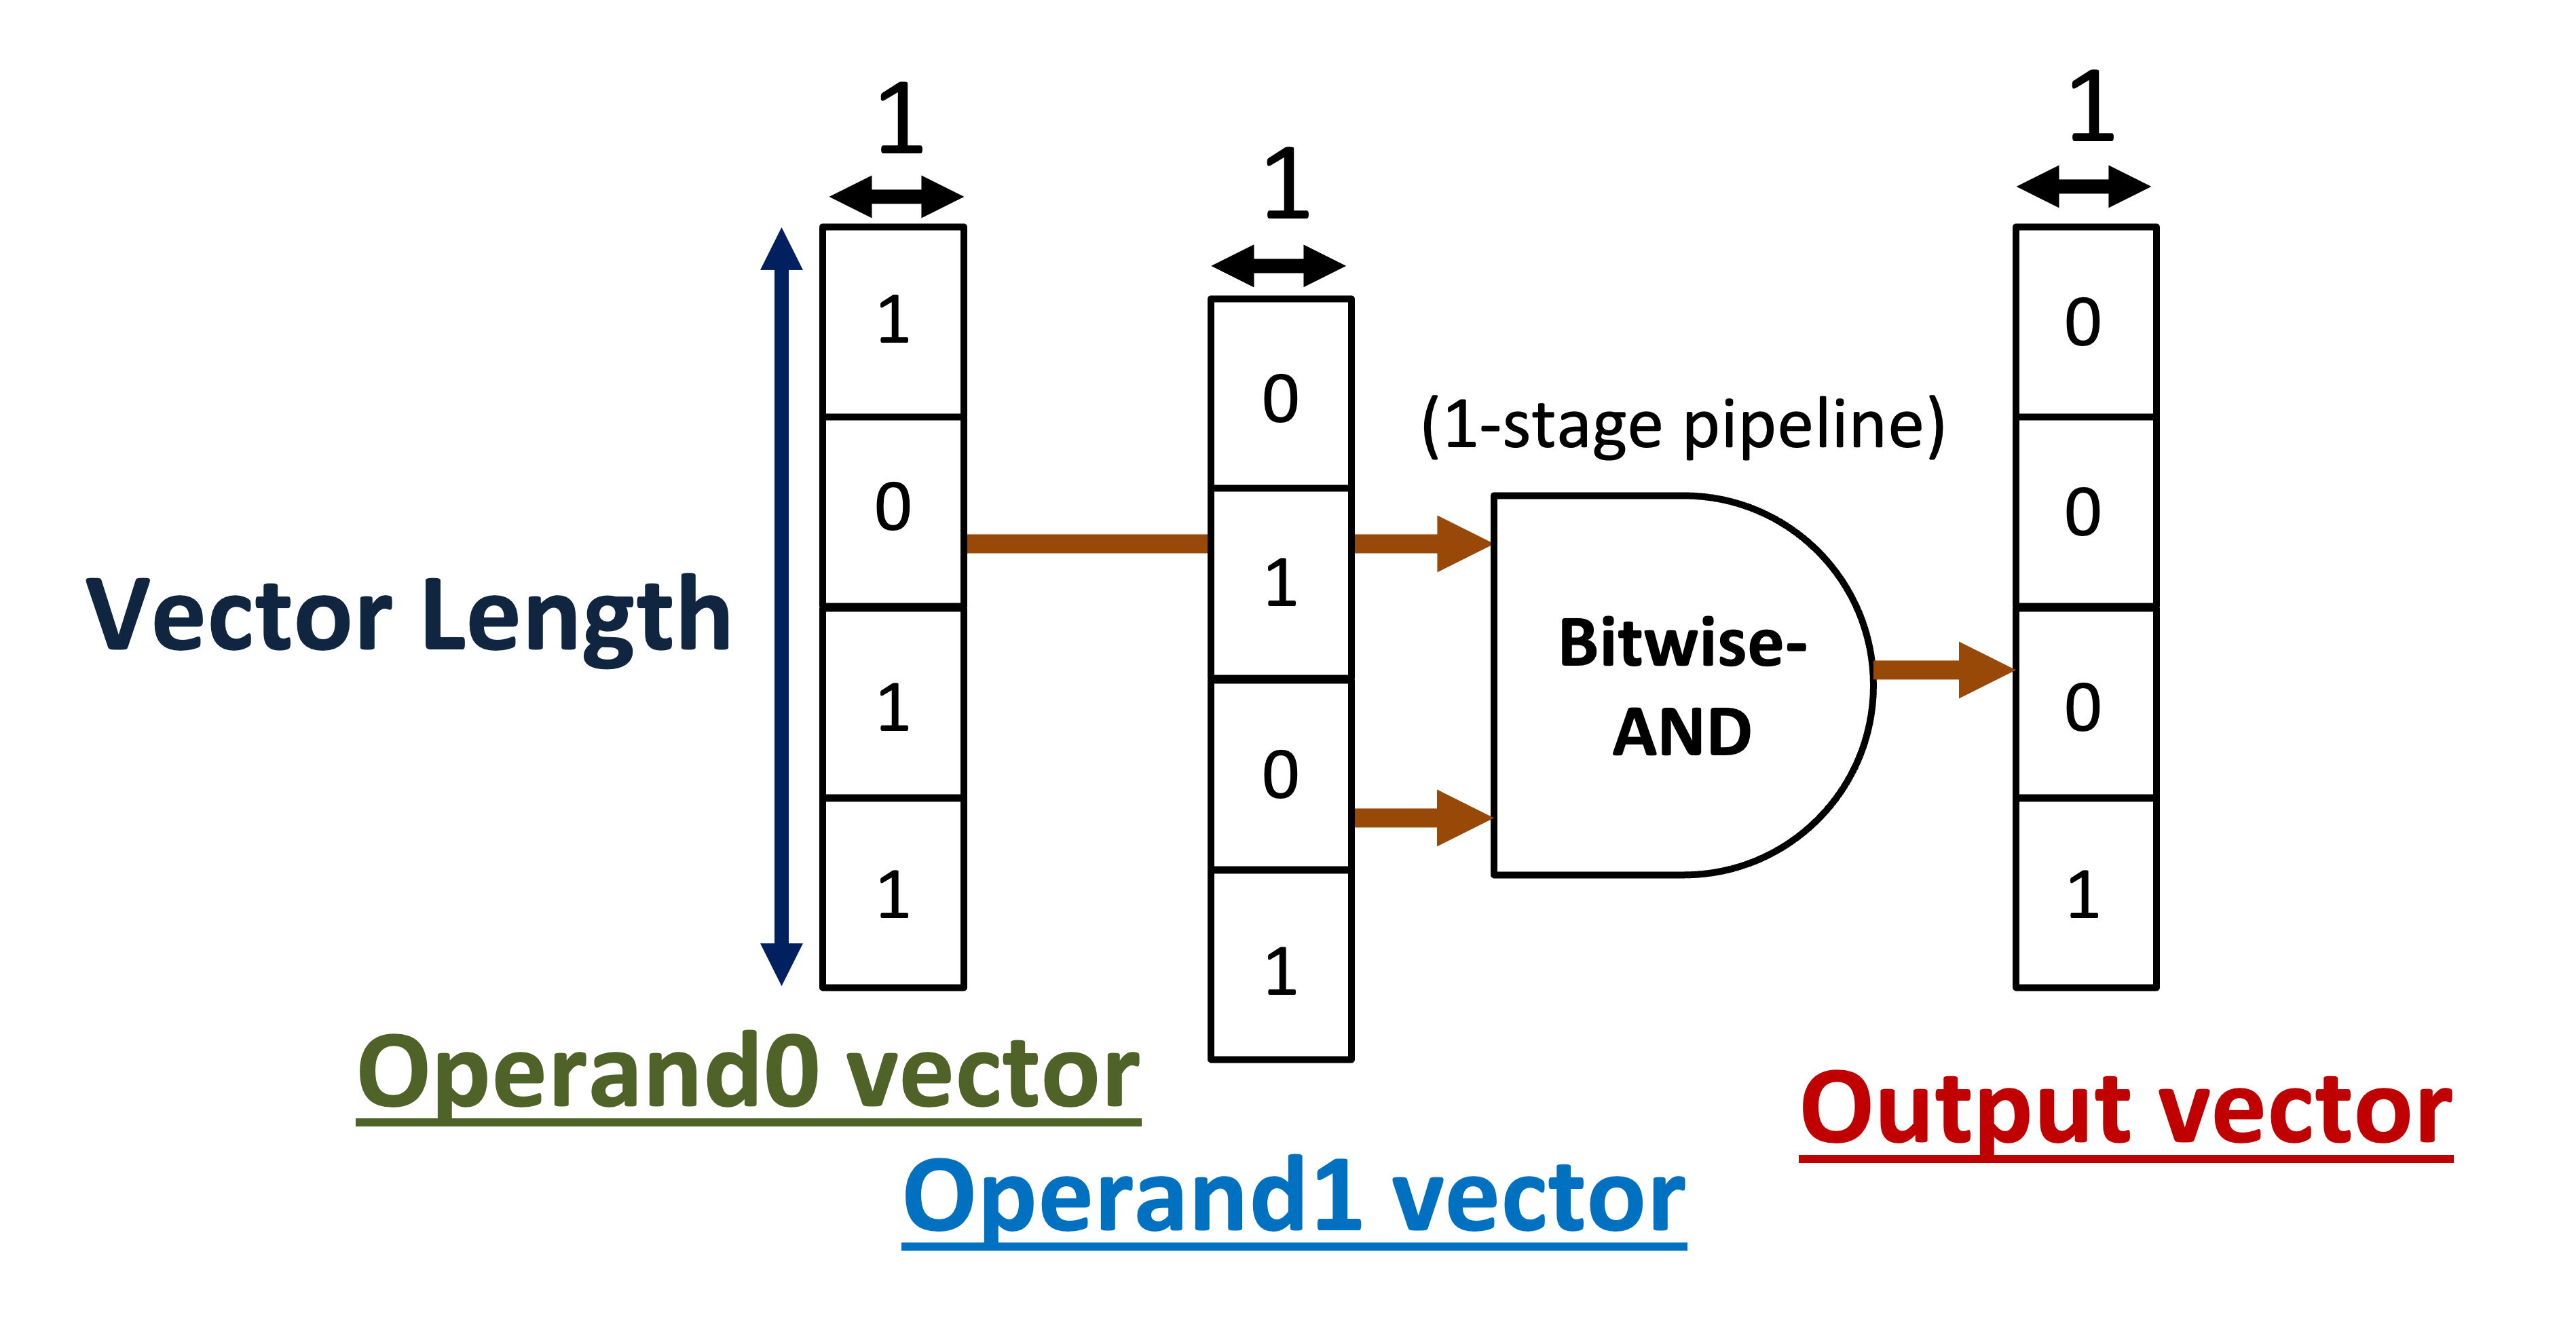
\includegraphics[width=\linewidth]{figures/bitmask_intersection.png}
    \caption{Bitmask intersection vector pipeline.}
    \label{fig:bitmask_intersection}
\end{figure}